% Drawing 12/06-2 -- folder 12, batch 06, archive page 117 (PDF page 118).
% Transcription: en bas à gauche, deux diagrammes des couples $(p, q)$, séparés par un trait vertical, sur un même axe horizontal. À gauche : un axe vertical gradué « $0$ », « $1$ », « $2$ », « $3$ », puis, au-dessus d'un trait horizontal, « $n-2$ », « $n-1$ », « $n$ » ; quatre croix sur chacune des rangées $0$ à $3$, puis quatre, deux et une croix aux rangées $n-2$, $n-1$, $n$. À droite : cinq croix sur l'axe et sur la rangée $1$, trois sur la rangée $2$, une sur la rangée $3$, les colonnes graduées « $2n-6$ », « $2n-5$ », « $2n-4$ », « $2n-3$ », « $2n-2$ ».
% Kind: two lattice diagrams of the pairs (p, q). Method 2 (schematic redraw from the facsimile). Status: ok.
% Notes: As counted on the page. Left diagram: the vertical axis, the horizontal axis (which runs on through the right diagram), the horizontal stroke that separates the rows 0 to 3 from the rows n-2, n-1, n; crosses: 4, 4, 4, 4 on the rows 0, 1, 2, 3 (the first of each on the vertical axis), then 4, 2, 1 on the rows n-2, n-1, n. Right diagram, after the vertical separating stroke: 5 crosses on the axis, 5 on the row 1, 3 on the row 2, 1 on the row 3, the columns labelled 2n-6, 2n-5, 2n-4, 2n-3, 2n-2 from left to right. Each cross is placed where he drew it. Left out: the formulas at the upper right of the crop (E_2 terms of the table above). Overlaid on the 400 dpi colour facsimile on 2026-11-12 (Opus 5.5): the axes, the separating strokes, every cross and every label lie on the page within about 1 mm; not changed. Redrawn 2026-11-12 (issue 128): to check again.
% Coordinates: 1 unit = 1 mm = 1/100 of the crop width (bbox in page fractions: [0.13, 0.67, 0.53, 0.835]).
% Redrawn by Claude (claude-fable-5-2), issue #128, 2026-11-12; not checked by a human; not compiled (no TeX in the session).
% Checked by Claude (claude-opus-5-5) 2026-11-12 (issue #128): overlaid on the 400 dpi colour facsimile; matches. Not compiled. Status: ok.
% Rights: reproduces part of the work -- behind RENDER_TRANSCRIPTS, never published by itself.
\documentclass[tikz,border=3pt]{standalone}
\usepackage{amsmath,amssymb}
\usetikzlibrary{patterns,arrows.meta}
\tikzset{pencil/.style={black!45}, struck/.style={black!35}, mpt/.style={circle,draw,inner sep=1.3pt}, pt/.style={circle,fill,inner sep=0.9pt}, opt/.style={circle,draw,fill=white,inner sep=1.1pt}}
\begin{document}
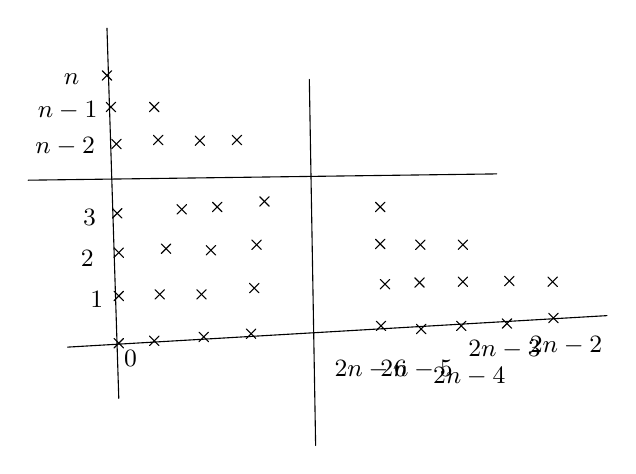
\begin{tikzpicture}[x=1mm,y=1mm,line cap=round,line join=round,font=\scriptsize]
\draw (17.5,-5) -- (19,-52);
\draw (12.5,-45.5) -- (81,-41.5);
\draw (7.5,-24.3) -- (67,-23.5);
\draw (43.2,-11.5) -- (44,-58);
\draw (18.4,-44.4) -- (19.6,-45.6);
\draw (18.4,-45.6) -- (19.6,-44.4);
\draw (22.9,-44.1) -- (24.1,-45.3);
\draw (22.9,-45.3) -- (24.1,-44.1);
\draw (29.2,-43.6) -- (30.4,-44.8);
\draw (29.2,-44.8) -- (30.4,-43.6);
\draw (35.2,-43.2) -- (36.4,-44.4);
\draw (35.2,-44.4) -- (36.4,-43.2);
\draw (18.4,-38.4) -- (19.6,-39.6);
\draw (18.4,-39.6) -- (19.6,-38.4);
\draw (23.6,-38.2) -- (24.8,-39.4);
\draw (23.6,-39.4) -- (24.8,-38.2);
\draw (28.9,-38.2) -- (30.1,-39.4);
\draw (28.9,-39.4) -- (30.1,-38.2);
\draw (35.6,-37.4) -- (36.8,-38.6);
\draw (35.6,-38.6) -- (36.8,-37.4);
\draw (18.4,-32.9) -- (19.6,-34.1);
\draw (18.4,-34.1) -- (19.6,-32.9);
\draw (24.4,-32.4) -- (25.6,-33.6);
\draw (24.4,-33.6) -- (25.6,-32.4);
\draw (30.1,-32.6) -- (31.3,-33.8);
\draw (30.1,-33.8) -- (31.3,-32.6);
\draw (35.9,-31.9) -- (37.1,-33.1);
\draw (35.9,-33.1) -- (37.1,-31.9);
\draw (18.2,-27.9) -- (19.4,-29.1);
\draw (18.2,-29.1) -- (19.4,-27.9);
\draw (26.4,-27.4) -- (27.6,-28.6);
\draw (26.4,-28.6) -- (27.6,-27.4);
\draw (30.9,-27.1) -- (32.1,-28.3);
\draw (30.9,-28.3) -- (32.1,-27.1);
\draw (36.9,-26.4) -- (38.1,-27.6);
\draw (36.9,-27.6) -- (38.1,-26.4);
\draw (18.1,-19.1) -- (19.3,-20.3);
\draw (18.1,-20.3) -- (19.3,-19.1);
\draw (23.4,-18.6) -- (24.6,-19.8);
\draw (23.4,-19.8) -- (24.6,-18.6);
\draw (28.7,-18.7) -- (29.9,-19.9);
\draw (28.7,-19.9) -- (29.9,-18.7);
\draw (33.4,-18.6) -- (34.6,-19.8);
\draw (33.4,-19.8) -- (34.6,-18.6);
\draw (17.4,-14.4) -- (18.6,-15.6);
\draw (17.4,-15.6) -- (18.6,-14.4);
\draw (22.9,-14.4) -- (24.1,-15.6);
\draw (22.9,-15.6) -- (24.1,-14.4);
\draw (16.9,-10.4) -- (18.1,-11.6);
\draw (16.9,-11.6) -- (18.1,-10.4);
\draw (51.7,-42.2) -- (52.9,-43.4);
\draw (51.7,-43.4) -- (52.9,-42.2);
\draw (56.8,-42.6) -- (58,-43.8);
\draw (56.8,-43.8) -- (58,-42.6);
\draw (61.9,-42.2) -- (63.1,-43.4);
\draw (61.9,-43.4) -- (63.1,-42.2);
\draw (67.7,-41.9) -- (68.9,-43.1);
\draw (67.7,-43.1) -- (68.9,-41.9);
\draw (73.6,-41.2) -- (74.8,-42.4);
\draw (73.6,-42.4) -- (74.8,-41.2);
\draw (52.2,-36.9) -- (53.4,-38.1);
\draw (52.2,-38.1) -- (53.4,-36.9);
\draw (56.6,-36.7) -- (57.8,-37.9);
\draw (56.6,-37.9) -- (57.8,-36.7);
\draw (62.1,-36.6) -- (63.3,-37.8);
\draw (62.1,-37.8) -- (63.3,-36.6);
\draw (68,-36.5) -- (69.2,-37.7);
\draw (68,-37.7) -- (69.2,-36.5);
\draw (73.5,-36.6) -- (74.7,-37.8);
\draw (73.5,-37.8) -- (74.7,-36.6);
\draw (51.6,-31.8) -- (52.8,-33);
\draw (51.6,-33) -- (52.8,-31.8);
\draw (56.7,-31.9) -- (57.9,-33.1);
\draw (56.7,-33.1) -- (57.9,-31.9);
\draw (62.1,-31.9) -- (63.3,-33.1);
\draw (62.1,-33.1) -- (63.3,-31.9);
\draw (51.6,-27.1) -- (52.8,-28.3);
\draw (51.6,-28.3) -- (52.8,-27.1);
\node[inner sep=1pt] at (13,-11.5) {\small $n$};
\node[inner sep=1pt] at (12.5,-15.5) {\small $n-1$};
\node[inner sep=1pt] at (12.2,-20) {\small $n-2$};
\node[inner sep=1pt] at (15.3,-29) {\small $3$};
\node[inner sep=1pt] at (15,-34.3) {\small $2$};
\node[inner sep=1pt] at (16.2,-39.5) {\small $1$};
\node[inner sep=1pt] at (20.5,-47) {\small $0$};
\node[inner sep=1pt] at (51,-48.3) {\small $2n-6$};
\node[inner sep=1pt] at (56.8,-48.3) {\small $2n-5$};
\node[inner sep=1pt] at (63.5,-49.3) {\small $2n-4$};
\node[inner sep=1pt] at (68,-45.8) {\small $2n-3$};
\node[inner sep=1pt] at (75.8,-45.3) {\small $2n-2$};
\end{tikzpicture}
\end{document}
